\section{Съществуващи решения и реализации}
В световен мащаб, идеята за проектиране на мебели посредством технологии за разширена реалност, не е нещо непознато. Компании в мебелния бизнес, като IKEA, Home Depot и др, предоставят подобни решения, които целят да улеснят клентите при избора им на предмети за дома.

IKEA Place е приложение на IKEA, което позволява на потребителите да ``поставят'' продуктите на IKEA във жилището си. Предлагано в App Store за iOS устройства, IKEA Place позволява визуализирането на обзавеждане, от дивани и лампи, до килими и маси, всички продукти в IKEA Place са 3D и в мащаб.Това помага на клентите да се уверят, че мебелта, която поръчват, е подходящият размер, с подходящия дизайн и функционалност. (Фиг. \ref{fig:ikea-place})

\begin{figure}[H]
    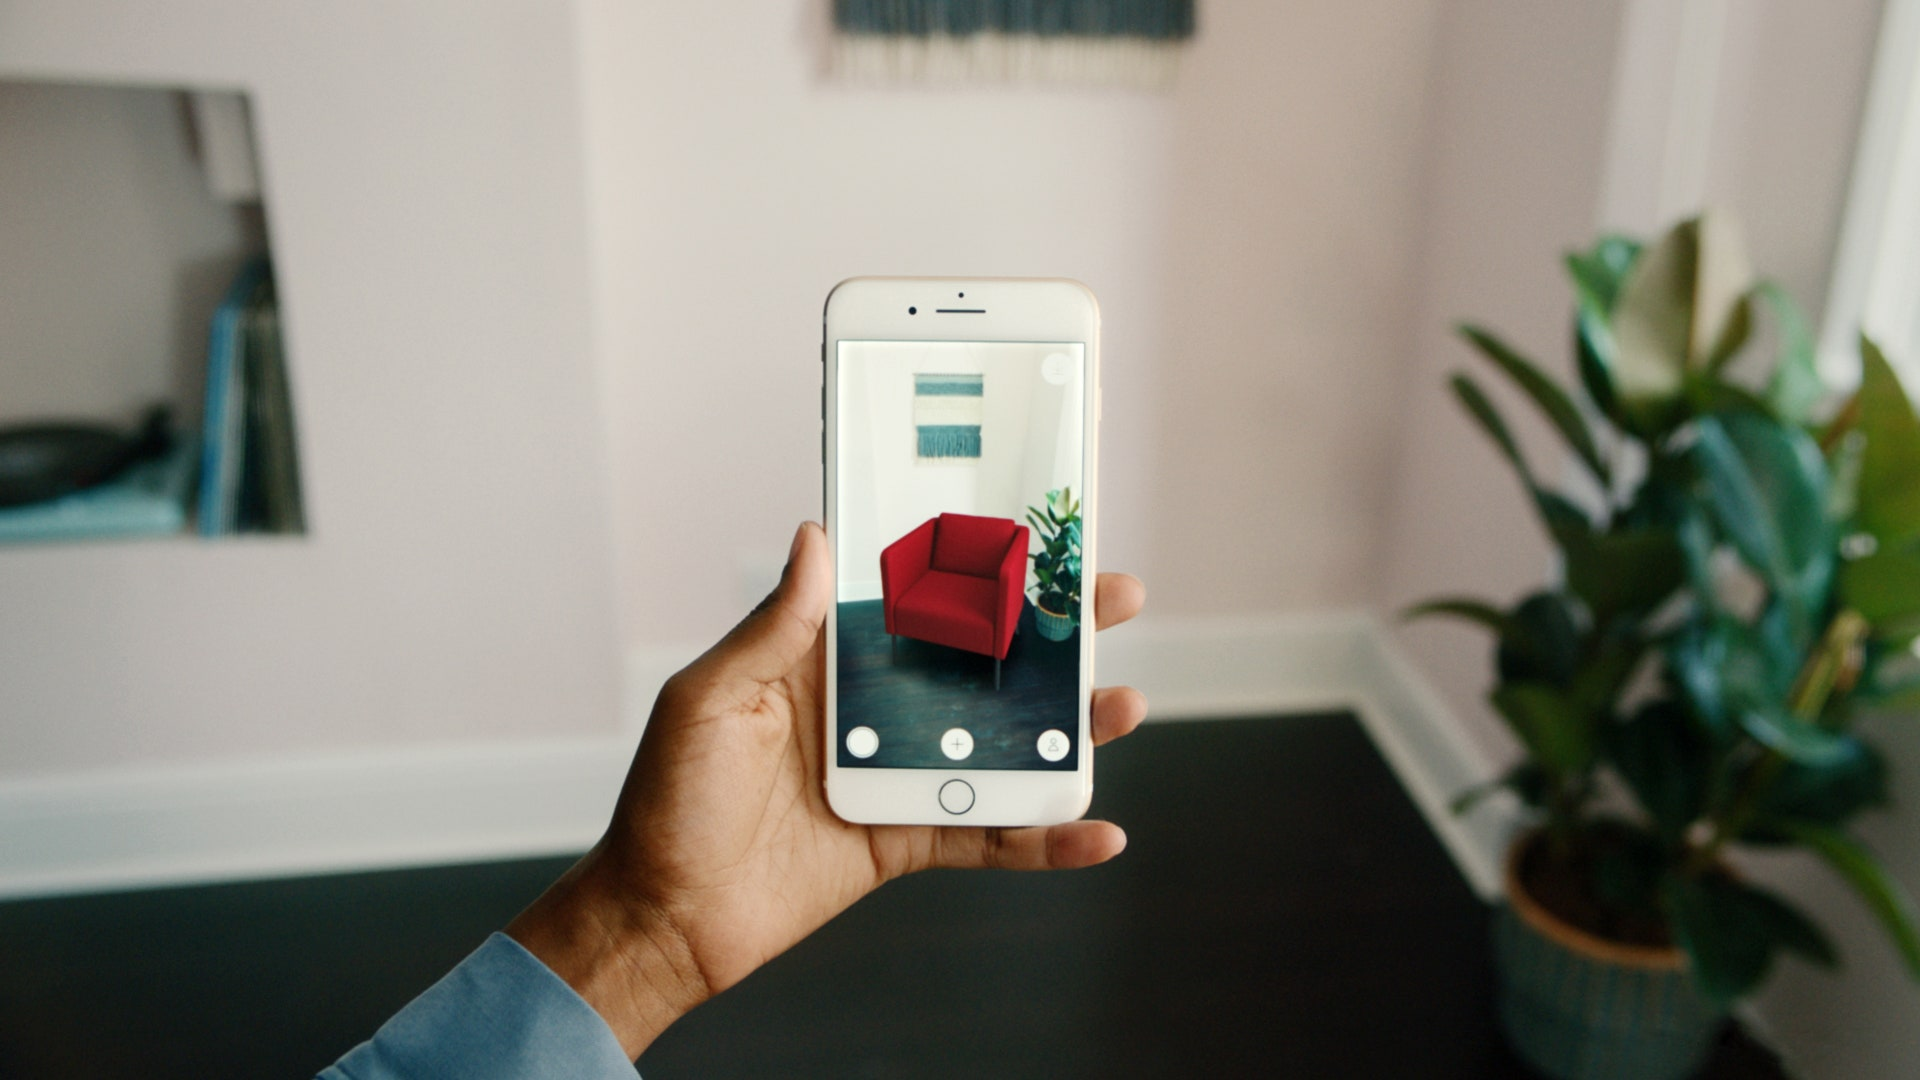
\includegraphics[width=1\textwidth]{ikea-place.jpeg}
    \centering
    \caption{Мобилното приложение IKEA Place}
    \label{fig:ikea-place}
\end{figure}

Приложението, разглеждано в тази дипломна работа, има преимуществото да се изпълнява и на Android, освен на iOS устройства.